\chapter{SPMonitor}

\todo{Add chapter introduction}

% This is the third result chapter which presents the first solution of the thesis.
% The solution is integrated into the overall concept introduced in Chapter 4 and
% it is technically based on the foundation described in Chapter 5.

% A thesis should provide at least two such solutions.

\todo{Explain purpose: maybe move motivation here; away from Analysis}

\section{Analysis}

\todo{Introduction to Analysis}

\subsection{Motivation}
The DrivingLicenseAuthorityKarlsruhe (DLAKa) wants to provide citizens with digital driving licenses,
which can, for example, be used to prove to a car rental company that they possess a valid driving license.
They hire the company ServiceProvider (SP) to develop and operate the system necessary for issuing and verifying
digital driving licenses. The contract specifies an initial payment for the development of the system
and afterward a yearly fee for the operation of the system.
After receiving the contract from DLAKa, SP starts designing the system
for DLAKa. Because SP has to operate the system on a fixed yearly budget,
they want to monitor the performance of the system to identify parts with excessive resource usage, which
incur additional costs. They identify the CPU and memory usage of the system as two technical metrics that should be monitored.
Additionally, DLAKa has asked them to provide the capability of monitoring business metrics for them.
DLAKa wants to know how many digital driving licenses are being issued and how often the issuance of a digital
driving license fails. To monitor both technical and business metrics, SP designs the ServiceProviderMonitor (SPMonitor) as a part
of the system for DLAKa which will provide all functionality for monitoring the specified metrics.

BestRental, a car rental company, has heard of DLAKa's plans for digital driving licenses
and wants to integrate them into its online rental system. Contrary to DLAKa, BestRental develops its
system in-house. Similarly to DLAKa, BestRental is interested in obtaining business metrics from its system.
They want to use these metrics to make business decisions like if they should increase the capacity of their fleet in the future.
For this purpose, BestRental designs an additional application called BestMonitor that will provide all the monitoring functionality.
In the beginning, they are only interested in one metric: How many active rentals are there?

For the design of SPMonitor, SP created two use cases: Present Metric and Collect Metric.
The relation of these use cases can be seen in the Use Case Diagram in Figure \ref{fig:use_case_monitoring_dlakaapp}.
Present Metric handles the use case of presenting the collected metrics to a user, this is described in Listing \ref{lis:use_case_description_present_metric}.
Collect Metric is concerned with how SPMonitor receives metrics for later presentation to a user, this is described in Listing \ref{lis:use_case_description_collect_metric}.

The metrics that will initially be monitored by SPMonitor are the number of issued digital driving licenses (NumDDL)
and the memory usage of the DLAKaApp (MemUse). The NumDDL metric is a business metric for DLAKa, while MemUse is
a technical metric that allows SP to monitor the performance of DLAKaApp.

\begin{figure}
	\centering
	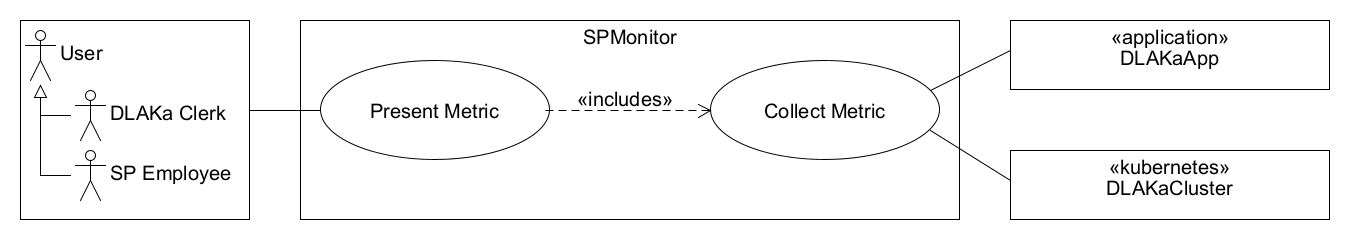
\includegraphics[width=\textwidth]{figures/2.1_use_case_spmonitor.png}
	\caption{Use Case Diagram: SPMonitor}
	\label{fig:use_case_monitoring_dlakaapp}
\end{figure}

\subsection{Use Case Present Metric}
\todo{Elaborate}

\begin{lstlisting}[caption = {Use Case Description: Present Metric}, label = {lis:use_case_description_present_metric}, style = kit-cm, language=]
Title: Present Metric

Primary Actors: DLAKa Clerk

Preconditions:
- SPMonitor has the NumDDL metric configured

Flow:
1. DLAKa Clerk opens the dashboard for the NumDDL metric
2. SPMonitor retrieves all stored values for the NumDDL metric
3. SPMonitor displays the values in a graph

Alternative Flows:
2a. SPMonitor has no values stored for the NumDDL metric
2a1. SPMonitor displays a message that the NumDDL metric has no stored values

Information Requirements:
- Values for the NumDDL metric
\end{lstlisting}

\subsection{Use Case Collect Metric}
\todo{Elaborate}

\begin{lstlisting}[caption = {Use Case Description: Collect Metric}, label = {lis:use_case_description_collect_metric}, style = kit-cm, language=]
Title: Collect Metric

Secondary Actors: DLAKaApp, DLAKaCluster

Preconditions:
- DLAKaApp is set up to collect the NumDDL metric
- DLAKaCluster is set up to collect the MemUse metric
- DLAKaApp is running inside of the DLAKaCluster
Postconditions:
- SPMonitor has values stored for NumDDL and MemUse

Flow:
1. SPMonitor sends a request to DLAKaApp for the NumDDL metric
2. DLAKaApp replies with a value for the NumDDL metric
3. SPMonitor receives the reply
4. SPMonitor stores the value for the NumDDL metric
5. SPMonitor sends a request to DLAKaCluster for the MemUse metric
6. DLAKaCluster replies with a value for the MemUse metric
7. SPMonitor receives the reply
8. SPMonitor stores the value for the MemUse metric

Alternative Flows:
2a. DLAKaApp replies with an error message
2a1. SPMonitor receives the error message
2a2. SPMonitor retries to request the NumDDL metric
6a. DLAKaCluster replies with an error message
6a1. SPMonitor receives the error message
6a2. SPMonitor retries to request the MemUse metric

Information Requirements:
- Value for the NumDDL metric
- Value for the MemUse metric
\end{lstlisting}

\todo{Summarize Analysis}

\section{Design}

\todo{Introduction for Design}
\todo{Explain criteria and derive from use case}

\begin{table}[]
\begin{tabular}{c|l}
Key & Criteria \\
\hline
C1 & Purpose \\
C2 & Licensing \\
C3 & Technical metrics \\
C4 & Business metrics \\
C5 & Kubernetes \\
C6 & Microsoft Azure \\
\end{tabular}
\caption{Selection criteria for monitoring tools}
\label{tab:monitoring_tool_criteria}
\end{table}

% NOTE: Many tools employ OpenTelemetry, especially for Business Metrics
\todo{Source for these tools}

\begin{table}[]
\begin{tabular}{l|c|c|c|c|c|c}
Name & C1 & C2 & C3 & C4 & C5 & C6 \\
\hline
Apache SkyWalking		 & Performance & Free & \cmark & \cmark & \cmark & \xmark \\
Cilium					 & Networking & Free & \cmark & \xmark & \cmark & \cmark \\
Datadog					 & SaaS & Paid & \cmark & \cmark & \cmark & \cmark \\
Dynatrace				 & PaaS & Paid & \cmark & \xmark & \cmark & \cmark \\
ELK						 & Searching & Paid & \cmark & \xmark & \cmark & \cmark \\
Honeycomb				 & Debugging & Paid & \cmark & \cmark & \cmark & \cmark \\
Instana					 & Incidence Management & Paid & \cmark & \xmark & \cmark & \cmark \\
Monasca					 & MaaS & Free & \cmark & \xmark & \cmark & \xmark \\
New Relic				 & PaaS & Paid & \cmark & \cmark & \cmark & \cmark \\
OpenSearch				 & Searching & Free & \cmark & \cmark & \cmark & \cmark \\
OpenTelemetry			 & Monitoring & Free & \cmark & \cmark & \cmark & \cmark \\
Prometheus/Grafana		 & Monitoring & Free/Paid & \cmark & \cmark & \cmark & \cmark \\
Scalyr					 & PaaS & Paid & \cmark & \xmark & \cmark & \xmark \\
SolarWinds				 & PaaS & Paid & \cmark & \xmark & \cmark & \cmark \\
Splunk					 & Resilience & Paid & \cmark & \cmark & \cmark & \cmark \\
Sumo Logic				 & Analytics & Paid & \cmark & \cmark & \cmark & \cmark \\
TICK					 & Time Series Data & Free/Paid & \cmark & \cmark & \cmark & \cmark \\
\end{tabular}
\caption{Comparison of monitoring tools}
\label{tab:monitoring_tool_comparison}
\end{table}

\todo{Elaborate final selection}

\todo{Explain SPS Architecture}

% Candidates:
% - Prometheus/Grafana
% - TICK
% - OpenSearch
% - OpenTelemetry

% The components that will be chosen for SPMonitor must fulfill a few requirements.
% These requirements are listed in Table \ref{tab:requirements}.
% Firstly, the solution should be scaleable to an arbitrary amount of monitored instances, and different workload sizes.
% Secondly, it should be possible to add new and different services in the future. This means that SPMonitor should be extensible.
% Thirdly, the components license model must permit free commercial use.
% Additionally, the components should be cloud agnostic, meaning that they are not bound to one vendor's specific cloud environment.
% Similarly, the components should not depend upon specific choices for the other components, so that the whole system can be freely designed.

% \begin{table}[h]
% \begin{tabular}{l|l}
% 	& Requirement       			\\
% \hline
% R1 	& Scalability 					\\
% R2 	& Extensibility       			\\
% R3 	& License			  			\\
% R4 	& Agnostic       				\\
% \end{tabular}
% \caption{Requirements for SPMonitor}
% \label{tab:requirements}
% \end{table}

% Note that the components are analyzed regarding their intended use.
% The result is, that a component might be listed as not fulfilling a requirement even though it would be possible
% to use the component in a way that fulfills the requirement. This is an important consideration for components
% that are part of a complete monitoring stack that offers components for all three types of components.
% Without this consideration, the fourth requirement would be violated.

% The components that were chosen in the end, can be seen in Figure \ref{fig:sps_spmonitor}.
% Grafana was chosen as the component for visualization together with Prometheus as the data source/sink.
% The combination of Grafana with Prometheus is an industry-standard solution that offers a lot of flexibility
% and functionality.
% Because Prometheus only stores metrics in memory and does not provide long-term storage,
% Grafana Mimir, with MinIO as a storage backend, was added to resolve this issue.
% The Grafana Agent was added as an additional data source because it provides an easy method
% of scraping performance metrics from Kubernetes Pods, which are then written to Prometheus for storage and analysis.

\begin{figure}
	\centering
	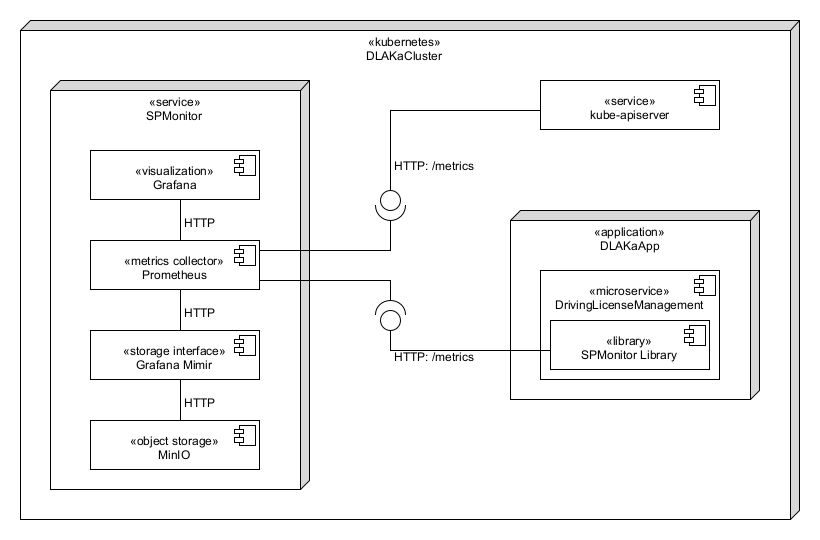
\includegraphics[width=\textwidth]{figures/sps_spmonitor.png}
	\caption{SystemPlusSoftware SPMonitor}
	\label{fig:sps_spmonitor}
\end{figure}

\section{Implementation}